\documentclass[10pt, a4paper]{article}
\usepackage{lrec2014}
\usepackage{graphicx}
\usepackage{hyperref}
\usepackage[utf8]{inputenc}
 

\title{Benchmarking multimedia technologies with the CAMOMILE platform: the case of Multimodal Person Discovery at MediaEval 2015}

\name{Johann Poignant$^1$, Hervé Bredin$^1$, Claude Barras$^1$,\\
     {\bf\large  Mickael Stefas$^2$, Pierrick Bruneau$^2$, Thomas Tamisier$^2$}
     }

\address{1. LIMSI, CNRS, Univ. Paris-Sud, Université Paris-Saclay, F-91405 Orsay, firstname.lastname@limsi.fr \\
		 2. LIST, Esch-sur-Alzette, Luxembourg,  firstname.lastname@list.lu\\}

\abstract{blabla \newline \Keywords{ }}



\begin{document}

\maketitleabstract

\section{Introduction}

For decades, NIST evaluation campaigns have been driving research in the field
of human language technology \cite{Martin2004}, recently followed by the CLEF \cite{Peters2002} and
ESTER/ETAPE \cite{Gravier2004} initiatives. The concept has been successfully transposed to
other research areas, such as image recognition (ImageNet Large Scale Visual
Recognition Challenge \cite{Russakovsky2015}), video (TRECVID \cite{Smeaton2006}) or multimedia indexing
(MediaEval \cite{Larson2015}). More generally, evaluation campaigns allow the assessment of
experimental research in fields where human perception and decision must be
reproduced by machine learning algorithms \cite{Geoffrois2008}.

The general workflow of \textit{à la NIST} evaluation campaigns comprises the
following stages \cite{Martin2004} specification of the task; definition of the evaluation
metric and provision of an automatic scoring software; design and annotation of
the training, development and evaluation corpora; definition of evaluation
rules, schedule, protocols and submission formats; sharing of participant
results through system descriptions and workshop communications.

Automatic scoring is made possible by the manual annotation of the data
according to the task definition. Costly and time-consuming, this annotation
step usually is the main bottleneck of evaluation campaigns. When addressing
new tasks in multimodal perception, it becomes challenging (if not impossible)
to pre-annotate the ever-increasing volume of multimedia data. A compromise
has been successfully explored in the TREC and TRECVid campaigns, where
the annotation of a small (but carefully chosen \cite{Yilmaz2006}) subset of the test data is
bootstrapped by the participants' submissions.

In this paper, we claim that the CAMOMILE collaborative annotation platform
(developed in the framework of the eponymous CHIST-ERA project) eases the
organization of multimedia technology benchmarks, automating most of the
campaign technical workflow and enabling collaborative (hence faster and
cheaper) annotation of the evaluation data. This is demonstrated through the
successful organization of a new multimedia task at MediaEval 2015, Multimodal
Person Discovery in Broadcast TV \cite{Poignant2015}.

\section{MediaEval 2015: Multimodal Person Discovery in Broadcast TV}

The objective of this new task is to make TV archives fully exploitable and
searchable through people indexing. Participants were provided with a
collection of TV broadcast recordings pre-segmented into shots. Each shot had
to be automatically tagged with the names of people both speaking and appearing
at the same time during the shot.

Since one cannot assume that biometric models of persons of interest are
available at indexing time, the main novelty of the task was that the list of
persons was not provided a priori. Biometric models (either voice or face)
could not be trained on external data. The only way to identify a person was by
finding their name in the audio (using speech transcription - ASR) or visual
(using optical character recognition - OCR) streams and associating them to the
correct person -- making the task completely unsupervised with respect to prior
biometric models.

To ensure that participants followed this strict ''no biometric supervision''
constraint, each hypothesized name had to be backed up by an ''evidence'': a
unique and carefully selected shot proving that the person actually holds this
name (e.g. a shot showing a text overlay introducing the person by their name).
In real-world conditions, this evidence would help a human annotator
double-check the automatically-generated index, even for people they did not
know beforehand.

Participants were provided with a fully functional baseline system, allowing
them to only focus on some aspects of the task (e.g. speaker diarization) while
still being able to rely on the baseline modules for the other ones (e.g.
optical character recognition). The task was evaluated as a standard
information retrieval task using a metric derived from mean average precision.
Eight teams managed to reach the submission deadline, amounting to a total of
70 submitted runs. For further details about the task, dataset and metrics, the
interested reader can refer to \cite{Poignant2015}.


\begin{figure*}[htb]
 \center 
 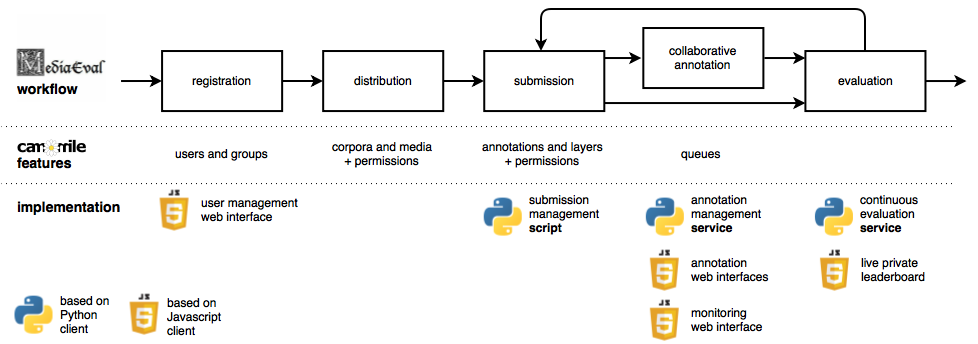
\includegraphics[width=1\linewidth]{figs/workflow.png}
 \centering
 \caption {Workflow automation with the CAMOMILE platform}
 \label{fig:archi}
\end{figure*}

\section{Person Discovery made easy with CAMOMILE}


The CAMOMILE platform was initially developed for supporting collaborative
annotation of multimodal, multilingual and multimedia data \cite{Poignant2016b}. The data model
was kept intentionally simple and generic, with four types of resources:
corpus, medium, layer and annotation.

A corpus is a set of media (e.g. the
evaluation corpus made of all test videos). An annotation is defined by a
fragment of a medium (e.g. a shot) with attached metadata (e.g. the name
of the current speaker). Finally, a layer is an homogeneous set of annotations,
sharing the same fragment type and the same metadata type (e.g. a complete run
submitted by one participant). All these resources are accessible through a
RESTful API (clients in Python and Javascript are readily available), with user
authentication and permission management.

A generic queueing mechanism is also
available on the CAMOMILE backend as a means to control the workflow. The
CAMOMILE platform is distributed as open-source software at the following
address: \url{http://github.com/camomile-project/camomile-server}.


\subsection{Automating the benchmarking workflow}

The upper part of Figure 1 depicts the technical workflow of the proposed
evaluation campaign.

The lower parts of Figure 1 summarize how we relied on the CAMOMILE platform
and its Python and Javascript clients to automate most of the workflow.

\textbf{Registration.} After the task was advertised through the MediaEval call for
participation, we relied on MediaEval standard registration procedure (i.e.
filling an online form and signing dataset usage agreements) to gather the list
of participating teams. Through a web interface, users and groups management
features of the CAMOMILE platform were used to create one group per team and
one user account for each team member.

\textbf{Distribution.}  Due to technical (limited internet bandwith) or copyright
concerns (datasets distributed by third parties), the development and
evaluation datasets were not distributed through the CAMOMILE platform.
Instead, ELDA and INA took care of sending the datasets to the participants.
Nevertheless, corresponding metadata for corpora (development and test sets)
and layers (for each video) were created as CAMOMILE resources with read
permissions for each team, then bound to a local copy of the videos.

\textbf{Submission.}  While the standard MediaEval submission procedure is to ask
participating teams to upload their runs into a shared online directory, we
chose to distribute to all participants a submission management tool, based on
the CAMOMILE Python client. This command line tool would automatically check
the format of the submission files, authenticate users with their CAMOMILE
credentials and creates a new layer (and associated annotations) for each
submission, with read/write permissions to (and only to) every team member.

\textbf{Evaluation.} For the duration of the submission period, a continuous
evaluation service based on the CAMOMILE Python client would update a live
leaderboard computed on a secret subset of the evaluation dataset -- providing
feedback to participants about the performance of their current submissions.

These four modules could easily be adapted to other benchmarking campaigns, as
long as the reference and submissions can follow the CAMOMILE data model.


\subsection{Collaborative annotation}

While the development dataset had already been annotated in the framework of
the past REPERE evaluation campaigns, the evaluation dataset was distributed by
INA without any annotation. Thanks to the CAMOMILE platform, we were able to
setup a collaborative annotation campaign where participants themselves would
contribute some time to annotate the evaluation dataset.

Two dedicated and complementary annotation web interfaces were developed, both
based on the CAMOMILE Javascript client. The first one is dedicated to the
correction of the ''pieces of evidence'' submitted by participants. For each correct
evidence, annotators had to draw a bounding box around the face of the person
and spellcheck their hypothesized name (firstname\_lastname). The second one
relies on the resulting mugshots to ask the annotator to decide visually if
the hypothesized person is actually speaking and visible during a video shot.

Both annotation interfaces relied on the CAMOMILE queueing feature, thanks to
a submission monitoring service that would continuously watch for new
submissions and update annotation queues accordingly. Moreover, a monitoring
interface was also accessible to the organizers to quickly gain insight into
the status of the annotation campaign (e.g. number of shots already annotated).

Table 1 summarizes the amount of work done during the annotation campaign.
7k+ ''evidence'' annotations were performed by 3 organizers while 66k+ ''label''
annotations were gathered from 20 team members -- leading to the annotation of
half of the evaluation corpus in less than a month.


\begin{table}[ht]
  \centering
  \begin{tabular}{|l|c|c|}
    \hline
                           & Evidence  & Label      \\
    \hline
    \hline
    \# annotators           & 3         & 20         \\
    \# annotations          & 7337      & 66089      \\
    Median duration        & 10.2s     & 4.4s       \\
    \hline
  \end{tabular}
  \caption{Amount and median duration of annotations for both interfaces}
  \label{tab:annotations}
\end{table}

While the annotation of ''evidence'' was done by the organizers themselves,
we wanted to guarantee the quality of the ''labels'' annotation done by the
participants themselves. To that end, each shot was required to be annotated at
least twice. Additional annotation of the same shot were requested until a
consensus was found. Tables 2 and 3 show that, thanks to a simple, focused and
dedicated ''label'' interface, the average number of required annotations
for each shot is close to the minimum (2).

\begin{table}[ht]
  \centering
  \begin{tabular}{|l|c|}
    \hline
                   		&  \# shots 			\\
    \hline
    \hline
	with 2+ annotations 	& 28231 (100.0\%) 	\\
	with consensus     	& 27873 ( 98.7\%) 	\\
	without consensus 	&   358 (  1.3\%) 	\\
    \hline
  \end{tabular}
  \caption{Proportion of shots with/without consensus}
  \label{tab:consensus1}
\end{table}


\begin{table}[ht]
  \centering
  \begin{tabular}{|l|c|}
    \hline
    \# annotations 		&  \# shots 			\\
    \hline
    \hline
	2             		& 22770 (81.7\%) \\
	3             		&  4257 (15.3\%) \\
	4             		&   658 ( 2.4\%) \\
	5+            		&   188 ( 0.6\%) \\
    \hline
  \end{tabular}
  \caption{Number of annotations per shot with consensus}
  \label{tab:consensus2}
\end{table}

A quick look at the few shots with 4 or more annotations reveals a few
ambiguous cases that were not forecast when designing the ''label'' annotation
interface: people singing or dubbed, barely audible speech, etc.


\section{Conclusion}

Relying entirely on the CAMOMILE annotation platform, a team of two people was
able to manage a large scale multimedia technology benchmark (10 teams,
70 submissions, 30k shots) -- including the development of the submission
management script, the leaderboard service and the whole annotation campaign.
Everything was hosted on a virtual private server with 2 cores and 2 GB of RAM
and resisted the load even during the peak submission time (right before the
deadline) and the concurrent collaborative annotation period.

All the script and interfaces related to this campaign are publicly available
on the CAMOMILE GitHub page. Though some were designed specifically for the
proposed MediaEval Person Discovery task, we believe that a significant part of
the approach is generic enough to be easily ported to a different task
where manual and automatic annotation of audio-visual corpora is involved.


\section{Acknowledgements}

This work was supported by France ''Agence Nationale de la Recherche''
(ANR) under grant ANR-12-CHRI-0006-01 and Luxembourg ''Fonds National de la
Recherche'' (FNR). We thank ELDA and INA for supporting the task with
development and evaluation datasets.

\section{Copyrights}

The Lan\-gua\-ge Re\-sour\-ce and Evalua\-tion Con\-fe\-rence (LREC) proceedings are published by the European Language Resources Association (ELRA). They include different media that may be used (i.e. hardcopy, CD-ROM, Internet-based/Web, etc.).

ELRA's policy is to acquire copyright for all LREC contributions. In assigning your copyright, you are not forfeiting your right to use your contribution elsewhere.  This you may do without seeking permission and is subject only to normal acknowledgement to the LREC proceedings.


\bibliographystyle{lrec2014}
\bibliography{publi}

\end{document}













